\documentclass[fr]{../../../../../../eplexam}

\usepackage{amsmath} % TODO

\usepackage{tikz}
\usepackage{pgfplots}
\pgfplotsset{
	compat=1.15,
	/pgf/declare function={
		% Warning: this function returns -2 for sqrtn(-4, 2)
		sqrtn(\x,\a) = \x/abs(\x) * abs(\x)^(1/\a);%FIXME maybe we could add the possibility to remove errors when x=0
	},
}
\usetikzlibrary{pgfplots.groupplots}

\DeclareMathOperator{\Res}{Res}

\hypertitle{Mathématiques}{3}{FSAB}{1103}{2018}{Août}{All}
{Nathan Jacques\and Jean-Martin Vlaeminck\thanks{Merci à Ulrich Winz, Martin Meerts et Baptiste Forget d'avoir donné si rapidement l'énoncé de l'examen}}
{Jean-François Remacle, Grégoire Winckelmans et Roland Keunings}

\section{EDP-caractéristiques}
On donne l'équation suivante sur le domaine \(\R^2\):
\[ y^{2n-1} \fpart{u}{x} - x^{2n-1} \fpart{u}{y} = U \frac{y^{4n-1}}{x^{2n+1}} \]
où \(n \ge 1 \), \(n \in \Z\), et \(U\) est une constante de même dimension que \(u\).

La caractéristique est telle que \(x(s) = s\), \(y(s) = s\) et \(u(s, 0) = 0\), pour \(s \ge 0\).

\begin{enumerate}
	\item Obtenez les équations des caractéristiques,
	et esquissez-les pour \(n=1\) et \(n=10\) pour différents \(s\).
	Aide: examinez le cas \(x=y\); \(2^{9/10}\approx 0.966\cdot 2^{1/2}\).
	Quelle forme particulière obtient-on pour \( n \to \infty \) ?
	\item Résolvez l'équation sur l'ensemble du domaine.
\end{enumerate}

\begin{solution}
On commence donc par utiliser la relation \( P \dif{y} = Q \dif{x} \) pour déterminer les caractéristiques:
\begin{align*}
y^{2n-1} \dif{y} &= -x^{2n-1} \dif{x} \\
\int_{y'=0}^{y} \frac{y'^{2n}}{2n} \dif{y'} &= \int_{x'=s}^{x} -\frac{x'^{2n}}{2n} \dif{x'} \\
y^{2n} &= -x^{2n} - (-s^{2n}) \\
x^{2n} + y^{2n} &= s^{2n}
\end{align*}
qui est l'équation d'un cercle dans différentes géométries non-euclidiennes,
ou un cas particulier de ce qu'on appelle en anglais une
\href{https://en.wikipedia.org/wiki/Superellipse}{superellipse}
en géométrie euclidienne.

Pour \( n = 1 \), on obtient \( x^2 + y^2 = s^2 \) qui est l'équation d'un cercle classique.
Pour \( n =2 \) (non demandé), on obtient \( x^4 + y^4 = s^4 \), qui est l'équation d'un \emph{squircle}.
Pour \( n = 10 \), on obtient une forme un peu plus pointue sur les coins du plan.
Pour \( n \to \infty \), la caractéristique devient un carré.
La figure~\ref{fig:q1_caracts} montre les caractéristiques pour les 4 cas mentionnés.

\begin{solfig}{q1_caracts}{Réseaux de caractéristiques de la question 1, pour \(n=1\), \(n=2\), \(n=10\) et \(n \to \infty \)}
	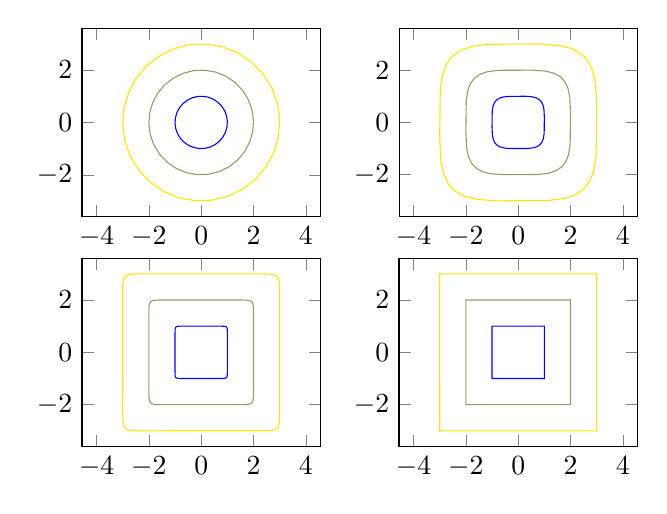
\begin{tikzpicture}
%	\begin{axis}[
%		axis equal,
%		domain=0:360,
%		variable=\t,
%		samples=20,
%		no markers,
%		colormap name=hot,
%		cycle list={[colors of colormap={0, 200, ..., 1000}]},
%	]
%	\foreach \n in {1, 2, 3}{
%		\foreach \s in {1, 2, 3}{
%			\addplot ({\s*sqrtn(cos(t), \n)}, {\s*sqrtn(sin(t), \n)});
%		}
%	}
%	\end{axis}
	\begin{groupplot}[
		group style={
			group size=2 by 2,
			vertical sep=15pt,
		},
		axis equal,
		width=0.38\textwidth,
		variable=\t,
		domain=2:362,
		samples=31,
		colormap name=hot,
		cycle list={[colors of colormap={0, 200, ..., 1000}]},
	]
	\pgfplotsinvokeforeach{1, 2, 10, 1000}{ % 1000 is nearly infinity
		\nextgroupplot
		\foreach \s in {1, 2, 3}{%
			\addplot+ (%
				{\s * sqrtn(cos(t), #1)},%
				{\s * sqrtn(sin(t), #1)}%
			);
		};
	};
	\end{groupplot}
	\end{tikzpicture}
\end{solfig}

Maintenant que les caractéristiques sont connues, continuons dans la résolution de l'équation.
On prend \(P \dif{u} = R \dif{x} \) comme relation de compatibilité:
\begin{align*}
y^{2n-1} \dif{u} &= U \frac{y^{4n-1}}{x^{2n+1}} \dif{x} \\
\dif{u} &= U \frac{y^{2n}}{x^{2n+1}} \dif{x} \\
&= U \frac{s^{2n} - x^{2n}}{x^{2n+1}} \dif{x} \\
\int_{u'=u(s, 0)}^{u(x, y)} \dif{u'} &= U \int_{t=s}^{t=x} \frac{s^{2n} - t^{2n}}{t^{2n+1}} \dif{t} \\
u(x, y) &= U \int_{t=s}^{t=x} \frac{s^{2n} - t^{2n}}{t^{2n+1}} \dif{t} \\
&= U \left[ -\frac{s^{2n}}{2n x^{2n}} - \log(t) \right]_{t=s}^{t=x} \\
&= -U\frac{s^{2n}}{2n x^{2n}} + U\frac{1}{2n} + U\log\left( \frac{s}{x} \right) \\
&= U \log\left(\frac{s}{x}\right) + U \frac{1}{2n} \left( 1 - \left(\frac{s}{x}\right)^{2n} \right)
\end{align*}
et donc,
\[
u(x, y) = U \log\left(\frac{s(x, y)}{x}\right) + U \frac{1}{2n} \left( 1 - \left(\frac{s(x, y)}{x}\right)^{2n} \right)
\qquad s(x, y) = \left(x^{2n}+y^{2n}\right)^{\frac{1}{2n}}.
\]

On peut vérifier que cette solution satisfait bien l'équation:
le calcul est long et fastidieux, plus compliqué que le calcul de cette solution\dots

Petite note: on peut aussi vérifier que les dimensions de chaque membre de l'équation sont cohérentes entre elles (en \([u]\cdot [x]^{2n-2}\)).
\end{solution}

\section{EDP-séparation des variables}
On considère l'équation de Laplace
\[ \nabla^2 u(r, \theta) = \frac{1}{r} \fpart{}{r} \left( r \fpart{u}{r} \right) + \frac{1}{r^2} \ffpart{u}{\theta} = 0 \]
dans un secteur d'anneau d'ouverture \(\beta\).
Les conditions limites sont \(u(a, \theta) = u(r, 0) = 0 \),
\( \fpart{u}{\theta} (r, \beta) = \frac{U}{\beta} \log\left( \frac{r}{a} \right) \)
et \( \fpart{u}{r} (b, \theta) = \frac{U}{b} g(\theta) \).

\begin{enumerate}
	\item Faites un dessin du domaine dans le plan \( (x, y) \) et \( (r, \theta) \)
	\item Résolvez cette équation par séparation des variables, en posant
	\[ u(r, \theta) = u_p (r, \theta) + u_h(r, \theta) \]
	avec \( u_p = \big(\log\left(\frac{r}{a}\right) + D\big) \big( A \theta + B \big) \)
	correspondant au mode zéro, et \(u_h\) correspondant au problème
	avec conditions limites homogènes en \(\theta\).
	Obtenez d'abord \( u_p \), puis \( u_h \).

	Énoncez clairement les intégrales à évaluer en fonction de \(g(\theta)\) pour déterminer les coefficients.
	\item Évaluez les intégrales pour
	\(g(\theta) = \sin \left(\frac{3\pi}{2} \frac{\theta}{\beta}\right) + \frac{\theta}{\beta} \)
\end{enumerate}

Aide: \( r^2 R'' + r R' - k^2 R = 0 \) a pour solution
\( R(r) = C \left(\frac{r}{L}\right)^k + D \left(\frac{r}{L}\right)^{-k} \),
où \( L \) est une grandeur caractéristique du problème.

\begin{solution}
La situation est présentée en figure~\ref{fig:q2_domains}.
\begin{solfig}{q2_domains}{Domaines et conditions}
	\begin{tikzpicture}
	\draw[thick, ->, >=latex] (-1, 0) -- (4, 0) node[right] {$x$};
	\draw[thick, ->, >=latex] (0, -1) -- (0, 3) node[above] {$y$};
	\draw[dkgreen]
		(2, 0) -- coordinate[midway] (lg1) (3, 0) arc (0:60:3) coordinate[midway] (lg2) coordinate (pt1)
		(2, 0) arc(0:60:2) coordinate[midway] (lg4) coordinate (pt2)
		(pt1) -- coordinate[midway] (lg3) (pt2)
	;
	\draw[dashed]
		(lg1) to[bend left] ++(-0.5, -0.5) node[left] {$u=0$}
		(lg2) to[bend left] ++(0.5, 0.5) node[right] {$\fpart{u}{r}(b, \theta)=\dfrac{U}{b}g(\theta)$}
		(lg3) to[bend left] ++(0, 1.2) node[right] {$\fpart{u}{\theta}(r, \beta)=\frac{U}{\beta} \log(r/a)$}
		(lg4) to[bend left] (1.2, 0.5) node[left] {$u=0$}
	;

	\draw[thick, ->, >=latex] (6, 0) -- (12, 0) node[right] {$r$};
	\draw[thick, ->, >=latex] (7, -1) -- (7, 3) node[above] {$\theta$};
	\draw[dkgreen] (7, 0) -- coordinate[midway] (lga) (10, 0) -- coordinate[pos=0.6] (lgb) (10, 2) -- coordinate[pos=0.3] (lgc) (7, 2) -- coordinate[pos=0.6] (lgd) cycle;
	\draw
		(lga) node[below] {$u=0$}
		(lgb) node[right] {$\fpart{u}{r}=\dfrac{U}{b}g(\theta)$}
		(lgc) node[above] {$\fpart{u}{\theta}=\frac{U}{\beta} \log(r/a)$}
		(lgd) node[left] {$u=0$}
	;
	
	\end{tikzpicture}
\end{solfig}

Pour la séparation des variables, on pose \(u(r, \theta) = R(r) \Theta(\theta) \) que l'on injecte dans l'équation:
\begin{align*}
\nabla^2 u(r, \theta) &= \frac{1}{r} \fpart{}{r} \left( r \fpart{}{r} (R(r)\Theta(\theta)) \right)
    + \frac{1}{r^2} \ffpart{}{\theta} (R(r)\Theta(\theta)) \\
0 &= \frac{1}{r}\fpart{}{r} \left(r \fpart{R}{r} \right) \Theta(\theta)
    + \frac{1}{r^2} \ffpart{\Theta}{\theta} R(r) \\
&= \frac{1}{r} \fdif{R}{r}(r) \Theta(\theta) + \ffdif{R}{r}(r) \Theta(\theta)
    + \frac{1}{r^2} R(r) \ffdif{\Theta}{\theta}(\theta) \\
0 &= \big( r^2 R''(r) + r R'(r) \big) \Theta(\theta) + R(r) \Theta''(\theta) \\
\frac{r^2 R''(r) + r R'(r)}{R(r)} &= -\frac{\Theta''(\theta)}{\Theta(\theta)} = \lambda
\end{align*}
où l'on a séparé notre équation en deux parties.

Comme d'habitude dans les problèmes opérants sur un domaine en cordonnées circulaires,
et comme conseillé par l'énoncé, on commence par examiner ce que donne le mode zéro
(càd la solution du problème pour \(\lambda=0\)) avant de regarder le restant:
en effet, dans un domaine circulaire, le mode zéro permet souvent d'éliminer
certaines conditions non homogènes ennuyantes, de sorte que le restant du problème
ait des conditions homogènes en \(\theta\).
Utilisons donc ce mode zéro.

Pour \(\lambda = 0\), la solution en \(\theta\) est linéaire (dérivée seconde nulle),
l'équation en \(r\) est \(r^2 R''(r) + r R'(r) = 0\) dont la solution\footnote{
En posant \(y(r)=R'(r)\), l'équation devient \(r y'(r)=-y(r)\) soit \(\fdif{y}{r}=-\frac{y}{r}\),
ce qui a pour solution (par séparation des variables) \(y(r)=\frac{C'}{r}\),
qu'il suffit d'intégrer pour trouver la solution \(R_p(r)=C\log(r)+D\).
}
est \(C\log(r)+D'\), et la combinaison des deux parties donne le mode zéro donné
\(u_p(r, \theta) = (A\theta+B)\left(\log(r/a) + D\right)\).

En \(r=a\) et en \(\theta=0\) on doit obtenir une solution nulle,
ce qui implique \(D=0\) et \(B=0\) respectivement, et donc
\(u_p(r, \theta) = A \theta \log\left(\frac{r}{a}\right)\).
La dérivée partielle selon \(\theta\) en \(\theta \beta\) vaut
\begin{align*}
\fpart{u_p}{\theta}(r, \beta) &= A \log\left(\frac{r}{a}\right) \\
&= \frac{U}{\beta} \log\left(\frac{r}{a}\right) \text{  par la troisième condition limite} \\
A &= \frac{U}{\beta}
\end{align*}
ce qui donne \(u_p = \frac{U \theta}{\beta} \log\left(\frac{r}{a}\right)\).
Le mode zéro satisfait alors les 2 conditions homogènes en \(\theta=0\) et \(r=a\),
et remplit la condition non homogène en \(\theta=\beta\); pour le restant du problème,
c'est-à-dire pour \(u_h\), la condition en \(\theta=\beta\) sera donc homogène.

Pour ce qui est du quatrième bord et de sa condition limite,
la solution particulière alias mode zéro y donne \(\fpart{u_p}{r}(b, \theta) = \frac{U\theta}{\beta b}\),
qu'il faut retrancher de la 4\ieme{} condition limite en \(r=b\) pour obtenir
la condition \(\fpart{u}{r}(b, \theta) = \frac{U}{b} g(\theta) - \frac{U\theta}{\beta}\)
à appliquer dans le restant du problème, c'est-à-dire la solution homogène \(u_h\).

Pour \(\lambda < 0\), la solution en \(\theta\) donne des exponentielles,
qui ne vont pas convenir pour notre résolution (voir cours pour une justification).

Pour \(\lambda = +k^2 > 0\), la solution en \(\theta\) donne des (co)sinus, ce qui est bien.
Les conditions limites sont, grâce au mode zéro, homogènes sur \(r=a\),
\(\theta=0\) et \(\theta=\beta\), et la condition non homogène restante est
\(\fpart{u_h}{r}(b, \theta) = \frac{U}{b} \left( g(\theta) - \frac{\theta}{\beta} \right) \).
Les équations du problème désormais homogène \(u_h\) sont
\[ \Theta_h''(\theta) + k^2 \Theta_h(\theta) = 0 \qquad \text{et} \qquad r^2 R_h''(r) + r R_h'(r) - k^2 R_h(r) = 0. \]

Pour ce qui est de \(\theta\), la solution est
\[ \Theta_h(\theta) = A \cos(k\theta) + B \sin(k\theta). \]
En \( \theta=0 \) \(u=0\) ce qui implique \(A=0\). En \(\theta = \beta\), on a
\[ \fpart{u_h}{\theta}(r, \beta) = R_h(r) \cdot \Theta_h'(\beta) = R_h(r) B k \cos(k \beta) = 0 \]
ce qui implique de choisir \(k\beta=\frac{(2n-1)\pi}{2}\) avec \(n\) entier
(on prend \(n=1, 2, \dots\) pour éviter d'avoir \(n=0\) et de le confondre avec le mode zéro).
Et donc, \(k_n = \frac{(2n-1)\pi}{2\beta}\).
On a donc une infinité de solutions homogènes \(u_{h, n}\) en fonction de \(k_n\),
qu'on pourra superposer pour satisfaire la condition non homogène et obtenir la solution complète.

En passant à \(R_{h,n}(r)\), son équation se résout, grâce à l'aide proposée, en
\[ R_{h,n}(r) = C_n \left(\frac{r}{a}\right)^{k_n} + D_n \left(\frac{r}{a}\right)^{-k_n}. \]
En appliquant la condition en \(r=a\), on obtient \(R_{h,n}(a)=C_n+D_n=0\) et donc
\(D_n=-C_n\) et \(R_{h,n}(r) = C_n \left( (r/a)^{k_n} - (r/a)^{-k_n}\right)\).
La solution homogène est constituée, comme toute solution d'un problème
résolu par séparation des variables, de la superposition des solutions
pour différentes valeurs de \(n\), soit
\[ u_h(r, \theta) = \sum_{n=1}^{\infty} C_n \left(
     \left(\frac{r}{a}\right)^{k_n} - \left(\frac{r}{a}\right)^{-k_n}
   \right) \sin(k_n \theta) \qquad k_n=\frac{(2n-1)\pi}{2\beta} \]
où il reste \og{}juste\fg{} à déterminer la valeur des constantes \(C_n\).
Pour cela, on utilise la 4\ieme{} condition limite et les propriétés d'orthogonalité des sinus et cosinus.

Sur le quatrième bord, la condition limite (pour les solutions homogènes!) s'écrit
\[ \fpart{u}{r}(b, \theta) = \sum_{n=1}^{\infty} \frac{C_n k_n}{a} \left(
     \left(\frac{b}{a}\right)^{k_n-1} + \left(\frac{b}{a}\right)^{-k_n-1}
   \right) \sin(k_n \theta) = \frac{U}{b} \left(g(\theta) - \frac{\theta}{\beta}\right). \]
Pour calculer le terme \(C_m\), on multiplie de part et d'autre par \(\sin(k_m\theta)\),
on intègre de \(0\) à \(\beta\), et on simplifie la somme (pour \(n\neq m\),
l'intégrale du \(n\)-ième terme sera nulle par orthogonalité, et pour \(n=m\),
l'intégrale vaudra \(\frac{\beta}{2}\)). Dès lors,
\[ \frac{C_m k_m}{b} \left( \left(\frac{b}{a}\right)^{k_m} + \left(\frac{b}{a}\right)^{-k_m} \right) \frac{\beta}{2}
   = \frac{U}{b} \int_{0}^{\beta} \left(g(\theta)-\frac{\theta}{\beta}\right) \sin(k_m\theta) \dif{\theta} \]
soit
\[ C_m = U \frac{2}{k_m \beta
     \left( \left(\frac{b}{a}\right)^{k_m} + \left(\frac{b}{a}\right)^{-k_m} \right)
   } \int_{0}^{\beta} \left(g(\theta)-\frac{\theta}{\beta}\right) \sin(k_m\theta) \dif{\theta}.
\]

Une fois les \(C_m\) connus, on peut écrire la solution de l'ensemble de l'équation comme
\[
u(r, \theta) = U \frac{\theta}{\beta} + \sum_{n=1}^{\infty} C_m \left(
  \left(\frac{r}{a}\right)^{k_m} - \left(\frac{r}{a}\right)^{-k_m}
\right) \sin(k_m \theta)
\]

Enfin, dans le cas particulier proposé,
\begin{align*}
\int_{0}^{\beta} \left(g(\theta)-\frac{\theta}{\beta}\right) \sin(k_m\theta) \dif{\theta}
&= \int_{0}^{\beta} \sin\left(\frac{3\pi}{2} \frac{\theta}{\beta} \sin(k_m \theta)\right) \\
&= \begin{cases}
\frac{\beta}{2} & \text{ si \(m=2\)} \\
0 & \text{ sinon}
\end{cases}
\end{align*}
ce qui donne
\[
C_m = \begin{cases}
U \frac{1}{k_2 \left( \left(\frac{b}{a}\right)^{k_2}
    + \left(\frac{b}{a}\right)^{-k_2} \right)} & \text{ si \(m=2\)} \\
0 & \text{ sinon}
\end{cases}
\]
et donc
\[
    u(r, \theta) = U \frac{\theta}{\beta} \log\left( \frac{r}{a} \right)
    + \frac{U}{k_2} \frac{
   	    \left(\frac{r}{a}\right)^{k_2} - \left(\frac{r}{a}\right)^{-k_2}
       }{
        \left(\frac{b}{a}\right)^{k_2} + \left(\frac{b}{a}\right)^{-k_2}
       } \sin(k_2 \theta) \qquad k_2=\frac{3\pi}{2\beta}.
\]
\begin{solfig}{q2_sol_part}{Graphe de la solution pour le cas particulier \(g(\theta) = \sin\left(\frac{3\pi\theta}{2\beta}\right)\)}
	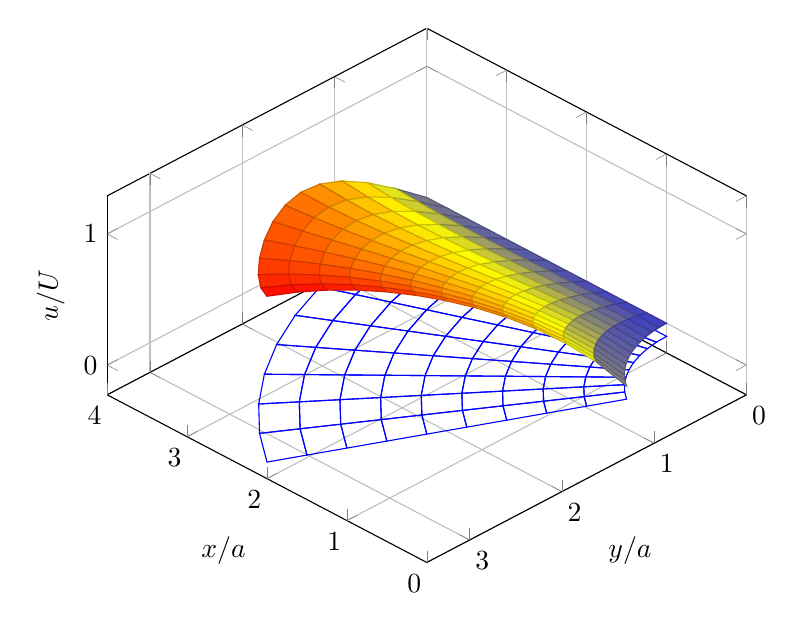
\begin{tikzpicture}
	\pgfmathsetmacro{\bbeta}{60};
	\pgfmathsetmacro{\a}{1};
	\pgfmathsetmacro{\b}{4};
	\pgfmathsetmacro{\kk}{(270/\bbeta)}
	\begin{axis}[
		xlabel={$x/a$},
		ylabel={$y/a$},
		zlabel={$u/U$},
		width=0.8\textwidth,
		grid,
		view/h=-135,
		view/v=50,
		no markers,
		xmin=0,
		ymin=0,
	]
	\addplot3+[
		mesh,
		variable=\r,
		variable y=\t,
		domain=\a:\b,
		domain y=0:\bbeta,
		samples=10,
		samples y=10,
	] ({r*cos(t)}, {r*sin(t)}, {-0.1});
	\addplot3+[
		surf,
		variable=\r,
		variable y=\t,
		domain=\a:\b,
		domain y=0:\bbeta,
		samples=13,
		samples y=13,
	] (%
		{r*cos(t)},%
		{r*sin(t)},%
		{((t/\bbeta)*ln(r/\a))%
		+ (1/\kk) * ( ((r/\a)^(\kk) - (r/\a)^(-\kk)) / ((\b/\a)^(\kk) + (\b/\a)^(-\kk)) ) * sin(\kk*t)%
		}%
	);
	\end{axis}
	\end{tikzpicture}
\end{solfig}
\end{solution}

\section{Analyse complexe 1}
Soit la fonction
\[ f(z) = \frac{z}{e^{z^2} -1} \]
\begin{itemize}
	\item Calculez le résidu de cette fonction en \( z = 0 \).
	\item Donnez tous les points singuliers de cette fonction et donnez leur type.
\end{itemize}

\begin{solution}
Tout d'abord, cette fonction n'est pas multiforme.
En effet, le numérateur n'est pas multiforme, \(z^2\) n'est pas multiforme,
et \(e^z\) est, de manière générale, pas multiforme non plus
(la seule chose qui compte pour une exponentielle c'est la valeur de la partie réelle
et celle de la partie imaginaire, pas (les multiples valeurs de) l'argument).

On se doute que les seuls endroits où la fonction peut avoir un comportement particulier sont en \(z=0\) (que l'on va analyser plus tard) et aux \(z\) tels que \(e^{z^2} = 1\) (annulation du dénominateur et donc pôle).

Pour le deuxième type de point, on pose \(z=x+\imag y\) qu'on injecte dans \(e^{z^2} = e^{x^2-y^2 + 2\imag x y} = 1\),
ce qui donne comme équations \(x^2=y^2\) et \(xy=k\pi\),
c'est-à-dire \(x=y\) ou \(x=-y\) et \(x^2 = k\pi\) avec \(k\in\Z\), soit les 4 familles de points
\[
\begin{array}{lcl}
	-x = y = \sqrt{k\pi} \quad k\in\N & \qquad & x = y = \sqrt{k\pi} \quad k\in\N \\
	x = y = -\sqrt{k\pi} \quad k\in\N & \qquad & x = -y = \sqrt{k\pi} \quad k\in\N \\
\end{array}
\]
Pour \(k\neq 0\), aucun de ces points ne cause la fonction à s'annuler au numérateur,
et donc il s'agit bien de pôles.
De même, vu que la fonction inverse \(g(z)=\frac{e^{z^2}-1}{z}\) s'annule en ces points,
mais que sa dérivée \(g'(z)=\frac{2z^2e^{z^2} - e^{z^2} + 1}{z^2}\) ne s'y annule pas,
il s'agit de pôles d'ordre 1.

Analysons maintenant le comportement de cette fonction en 0.

\(0\) est un pôle d'ordre 1 de la fonction. En effet, la fonction inverse, \(g(z)\),
admet un développement en série de Laurent
\[ g(z) = \frac{1 + z^2 + \frac{z^4}{2!} + \frac{z^6}{3!} + \dots - 1}{z} = z + \frac{z^3}{2!} + \frac{z^5}{3!} + \dots \]
qui est en fait une série de Taylor, et qui montre qu'en \(0\), la fonction vaut \(0\).
Par contre, la dérivée de cette fonction n'est pas nulle, ce qui signifie que
le zéro de \(g(z)\) est d'ordre 1, et donc que le pôle de \(f(z)\) est d'ordre 1.

Pour le calcul du résidu, il faut alors calculer
\(\lim\limits_{z\to 0} z\cdot f(z) = \frac{z^2}{e^{z^2}-1} = \frac{r(z)}{s(z)}\)
avec \(r(z)=z^2\) et \(s(z)=e^{z^2}-1\).
Pour cela, on applique la règle de Bernouilli (ou de L'Hospital):
les conditions d'application sont en effet satisfaites (\(r\) et \(s\) holomorphes).
On effectue:
\[
  \Res(f; 0) = \lim\limits_{z\to 0} \frac{z^2}{e^{z^2}-1} = \lim\limits_{z\to 0}
  \frac{2z}{2ze^{z^2}} = \lim\limits_{z\to 0} \frac{1}{e^{z^2}} = \frac{1}{1} = 1
\]
De manière plus détaillée, on remarque que
\[ zf(z) = \frac{z^2}{e^{z^2}-1} = \frac{r(z)}{s(z)} \]
avec
\[ r(z) = z^2 = 0 + (z-0)\cdot \underbrace{0}_{r'(0)} + (z-0)^2 \cdot \underbrace{1}_{r''(0)/2} + (z-0)^2 \cdot \underbrace{r_2(z)}_{r_2(0)=0} \]
et
\[ s(z) = e^{z^2} - 1 = z^2 + \frac{z^4}{2!} + \frac{z^6}{3!} + \dots = 0 + (z-0) \cdot \underbrace{0}_{s'(0)} + (z-0)^2 \cdot \underbrace{1}_{s''(0)/2} + (z-0)^2 \cdot \underbrace{s_2(z)}_{s_2(0)=0} \]
ce qui permet d'écrire
\begin{align*}
\lim\limits_{z\to 0} z f(z) &= \frac{r(z)}{s(z)} = \lim\limits_{z\to 0} \frac{0 + (z-0) \cdot 0 + (z-0)^2 \cdot 1 + (z-0)^2 r_2(z)}{0 + (z-0) \cdot 0 + (z-0)^2 \cdot 1 + (z-0)^2 s_2(z)} \\
&= \lim\limits_{z\to 0} \frac{1 + r_2(z)}{1 + s_2(z)} = \frac{1}{1} = 1.
\end{align*}
\end{solution}

\section{Analyse complexe 2}
Évaluez l'intégrale suivante à l'aide du théorème des résidus. Les lemmes de Jordan ne sont \strong{pas} donnés.
\[ \int_{0}^{2\pi} \frac{\cos(x)}{5+4\cos(x)} \dif{x} \]

\begin{solution}
En posant \( \cos(x) = \tfrac{z+\tfrac{1}{z}}{2} \) avec \(z = 1 \e^{\imag x}\),
l'intégrale devient une intégrale de contour autour du cercle \(\mathcal{C}\) de rayon 1
centré à l'origine dans le plan complexe, d'une fonction \( f(z) \) à déterminer.
On obtient, en portant \(z\) dans l'intégrale,
\begin{align*}
I &= \int_{0}^{2\pi} \, \frac{\cos(x)}{5+4\cos(x)} \dif{x} \\
&= \int_\mathcal{C} \, \frac{1}{2 \vphantom{\left(z+\tfrac{1}{z}\right)}}
   \frac{z + \tfrac{1}{z}}{5+2\left(z+\tfrac{1}{z}\right)}
   \frac{1}{\imag z} \dif{z} \\
&= \int_\mathcal{C} \, \frac{1}{2\imag} \frac{z^2 + 1}{z(5z+2z^2+2)} \dif{z} \\
&= \int_\mathcal{C} \, \frac{1}{4\imag \vphantom{\tfrac{5}{2}}}
   \frac{z^2 + 1}{z(z^2+\tfrac{5}{2}z+1)} \dif{z} \\
&= \int_\mathcal{C} \, f(z) \dif{z}
\end{align*}
où l'on définit la fonction complexe
\[ f(z) = \frac{1}{4\imag \vphantom{z(z^2+\tfrac{5}{2}z+1)}} \frac{z^2 + 1}{z(z^2+\tfrac{5}{2}z+1)} \]
que l'on va analyser.

A noter que l'on a pas besoin, ici, de déterminer une quelconque coupure;
la fonction n'est pas multiforme, donc elle n'a qu'une seule branche.

Le dénominateur se factorise en
\[ f(z) = \frac{1}{4\imag \vphantom{z(z+\tfrac{1}{2})(z+2)}} \frac{z^2 + 1}{z(z+\tfrac{1}{2})(z+2)} \]
et la fonction n'a donc que 3 points singuliers: les pôles simples en \(z=0\),
\(z=-\frac{1}{2}\) et \(z=-2\). De ces pôles, seuls \(0\) et \(-\frac{1}{2}\)
sont à l'intérieur du domaine défini par le contour d'intégration \(\mathcal{C}\).
Il faut donc calculer le résidu de \(f\) en ces points. Pour un pôle d'ordre \(n\):
\[ \Res(f; a) = \frac{1}{(n-1)!} \lim\limits_{z\to a} \fnpart{}{z}{n-1} ((z-a)^n f(z)) \]
et donc, pour un pôle d'ordre \(1\),
\begin{align*}
\Res(f; a) &= \lim\limits_{z\to a} (z-a)f(z) \\
\Res(f; 0) &= z \cdot f(z) \big\rvert_{0} = \frac{1}{4\imag} \frac{1}{\tfrac{1}{2} \cdot 2} = \frac{1}{4\imag} \\
\Res\left(f; -\frac{1}{2}\right) &= \left(z+\frac{1}{2}\right) f(z) \rvert_{-\frac{1}{2}}
= \frac{1 \vphantom{1+\tfrac{1}{4}}}{4\imag \vphantom{\tfrac{-1}{2} \tfrac{3}{2}}}
\frac{1+\tfrac{1}{4}}{\tfrac{-1}{2} \tfrac{3}{2}}
= \frac{1}{4\imag} \frac{5}{-3} = \frac{-5}{12\imag}.
\end{align*}

Dès lors, on peut écrire
\begin{align*}
I &= 2\pi \imag \cdot \left( \Res(f; 0) + \Res\left(f; -\frac{1}{2} \right)\right) \\
&= 2\pi \imag \left(\frac{1}{4\imag} - \frac{5}{12\imag} \right) \\
&= -\frac{4\pi\imag}{12\imag} = -\frac{\pi}{3}
\end{align*}
ce qui donne finalement
\[ \int_{0}^{2\pi} \frac{\cos(x)}{5+4\cos(x)} \dif{x} = -\frac{\pi}{3} \]

\end{solution}

\end{document}
